\documentclass[../../Main.tex]{subfiles}
\begin{document}
  For a better understanding of the use cases, I'd like to include the corresponding activity diagrams beneath each specification.
  \begin{table}[H]
    \centering
    \begin{tabular}{|
    >{\columncolor[HTML]{32CB00}}l |lll|}
    \hline
    \textbf{Usecase code}       & \multicolumn{1}{l|}{UC001} & \multicolumn{1}{l|}{\textbf{Usecase name}} & Social login \\ \hline
    \textbf{Actor}              & \multicolumn{3}{l|}{User}                                                              \\ \hline
    \textbf{Pre-condition}       & \multicolumn{3}{l|}{At least have 1 social account}                                    \\ \hline
    \textbf{Main flow of event} & \multicolumn{3}{l|}{
              \begin{tabular}{|
                >{\columncolor[HTML]{FFFFFF}}p{2cm}|p{3cm}|p{6cm}|}
                    \hline
                    \cellcolor[HTML]{F56B00}\textbf{No} & \cellcolor[HTML]{F56B00}\textbf{Actor} & \cellcolor[HTML]{F56B00}\textbf{Action} \\ \hline
                    \textbf{1}                          & User                                   &  Select social login type    \\ \hline
                    \textbf{2}                          & System                                       &  Redirect to authorize\\ \hline
                    \textbf{3}                          & Auth0                                       &  Redirect to login and authorization form  \\ \hline
                    \textbf{4}                          & User                                       & Authenticate and consent                                         \\ \hline
                    \textbf{5}                          & Auth0                                       & Redirect with single use authorization code\\ \hline
                    \textbf{6}                          & System                                  & Send code clientId and credentials to get oauth token\\ \hline
                    \textbf{7}                          & Auth0                                   & Verify code, cliendId, credentials \\ \hline
                    \textbf{8}                          & Auth0                                   & Send idToken, access token and refresh token\\ \hline
                    \textbf{9}                          & System                                  & Authenticate the idToken or access token\\ \hline
                    \textbf{10}                          & System                                  & Assign encKey for user\\ \hline
                    \textbf{11}                          & System                                  & Send shares \\ \hline
                    \textbf{12}                          & System                                  & Contruct the encKey \\ \hline
                    \textbf{13}                          & System                                  & Construct the private Key \\ \hline
              \end{tabular}
    } \\ \hline
    \textbf{Alternative flow of event} & \multicolumn{3}{l|}{
              \begin{tabular}{|
                >{\columncolor[HTML]{FFFFFF}}p{2cm}|p{3cm}|p{6cm}|}
                    \hline
                    \cellcolor[HTML]{F56B00}\textbf{No} & \cellcolor[HTML]{F56B00}\textbf{Actor} & \cellcolor[HTML]{F56B00}\textbf{Action} \\ \hline
                    \textbf{5b}                          & Auth0    &  Return error if the authenticate and consent fail or rejected\\ \hline
                    \textbf{8b}                          & Auth0    &  Response with error because fail in verification\\ \hline
              \end{tabular}
    }
    \end{tabular}
      \caption{Sign up specification}
      \label{sign-up-specification}
    \end{table}
    \begin{figure}[H]
     \centering
     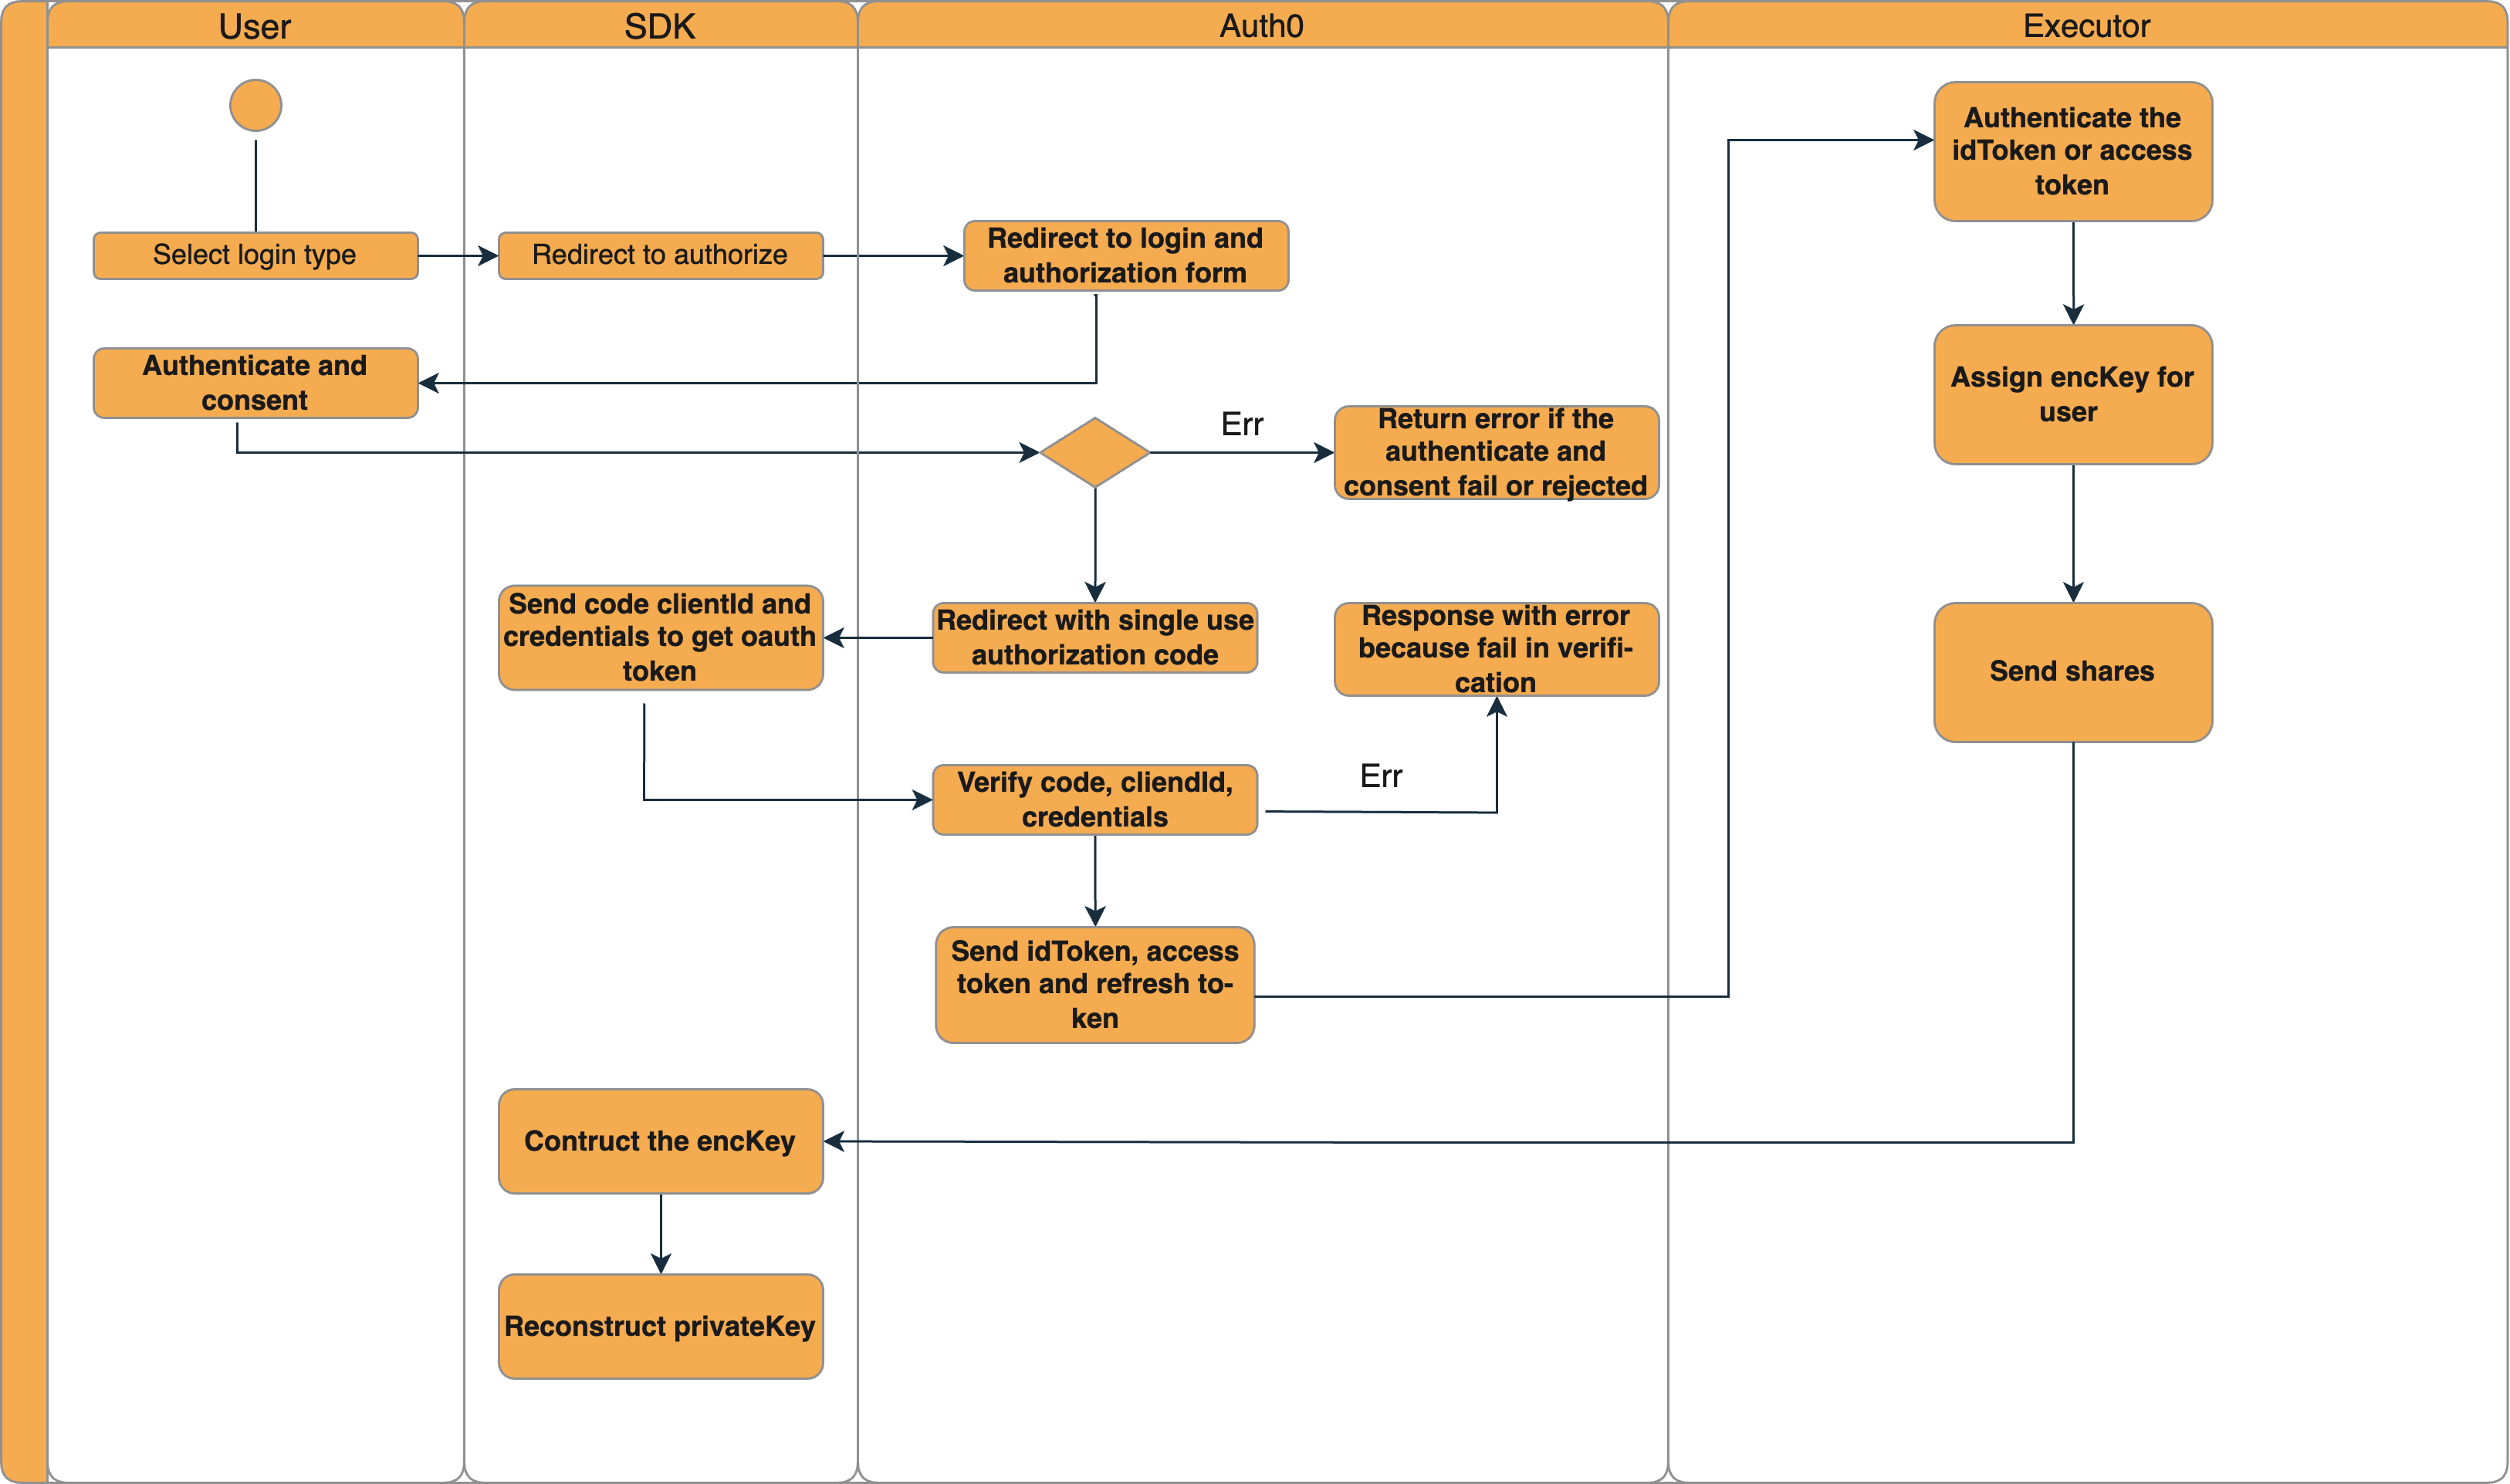
\includegraphics[scale=0.14]{Figure/sign-up-activity.png}
     \caption{Signing up activity}
        \label{fig:sign-up-activity}
    \end{figure}
    Figure \ref{fig:sign-up-activity} is an activity diagram that illustrates the process, how users interact with the system, and the connections between the components. The SDK acts as a bridge between users and the remainder of the system, while Executors and Auth0 validate users' identities. In addition, executors assign and provide the requirements for user encKey and private key construction.

  \begin{table}[H]
    \centering
    \begin{tabular}{|
    >{\columncolor[HTML]{32CB00}}l |lll|}
    \hline
    \textbf{Usecase code}       & \multicolumn{1}{l|}{UC001} & \multicolumn{1}{l|}{\textbf{Usecase name}} & Social login \\ \hline
    \textbf{Actor}              & \multicolumn{3}{l|}{User}                                                              \\ \hline
    \textbf{Pre-condition}       & \multicolumn{3}{l|}{At least have 1 social account}                                    \\ \hline
    \textbf{Main flow of event} & \multicolumn{3}{l|}{
              \begin{tabular}{|
                >{\columncolor[HTML]{FFFFFF}}p{2cm}|p{3cm}|p{6cm}|}
                    \hline
                    \cellcolor[HTML]{F56B00}\textbf{No} & \cellcolor[HTML]{F56B00}\textbf{Actor} & \cellcolor[HTML]{F56B00}\textbf{Action} \\ \hline
                    \textbf{1}                          & User                                   &  Select social login type    \\ \hline
                    \textbf{2}                          & System                                       &  Redirect to authorize\\ \hline
                    \textbf{3}                          & Auth0                                       &  Redirect to login and authorization form  \\ \hline
                    \textbf{4}                          & User                                       & Authenticate and consent                                         \\ \hline
                    \textbf{5}                          & Auth0                                       & Redirect with single use authorization code\\ \hline
                    \textbf{6}                          & System                                  & Send code clientId and credentials to get oauth token\\ \hline
                    \textbf{7}                          & Auth0                                   & Verify code, cliendId, credentials \\ \hline
                    \textbf{8}                          & Auth0                                   & Send idToken, access token and refresh token\\ \hline
                    \textbf{9}                          & System                                  & Authenticate the idToken or access token\\ \hline
                    \textbf{10}                          & System                                  & Send shares \\ \hline
                    \textbf{11}                          & System                                  & Contruct the encKey \\ \hline
                    \textbf{12}                          & System                                  & Construct the private Key \\ \hline
              \end{tabular}
    } \\ \hline
    \textbf{Alternative flow of event} & \multicolumn{3}{l|}{
              \begin{tabular}{|
                >{\columncolor[HTML]{FFFFFF}}p{2cm}|p{3cm}|p{6cm}|}
                    \hline
                    \cellcolor[HTML]{F56B00}\textbf{No} & \cellcolor[HTML]{F56B00}\textbf{Actor} & \cellcolor[HTML]{F56B00}\textbf{Action} \\ \hline
                    \textbf{5b}                          & Auth0    &  Return error if the authenticate and consent fail or rejected\\ \hline
                    \textbf{8b}                          & Auth0    &  Response with error because fail in verification\\ \hline
              \end{tabular}
    }
    \end{tabular}
      \caption{Sign in specification}
      \label{sign-in-specification}
    \end{table}
    \begin{figure}[H]
     \centering
     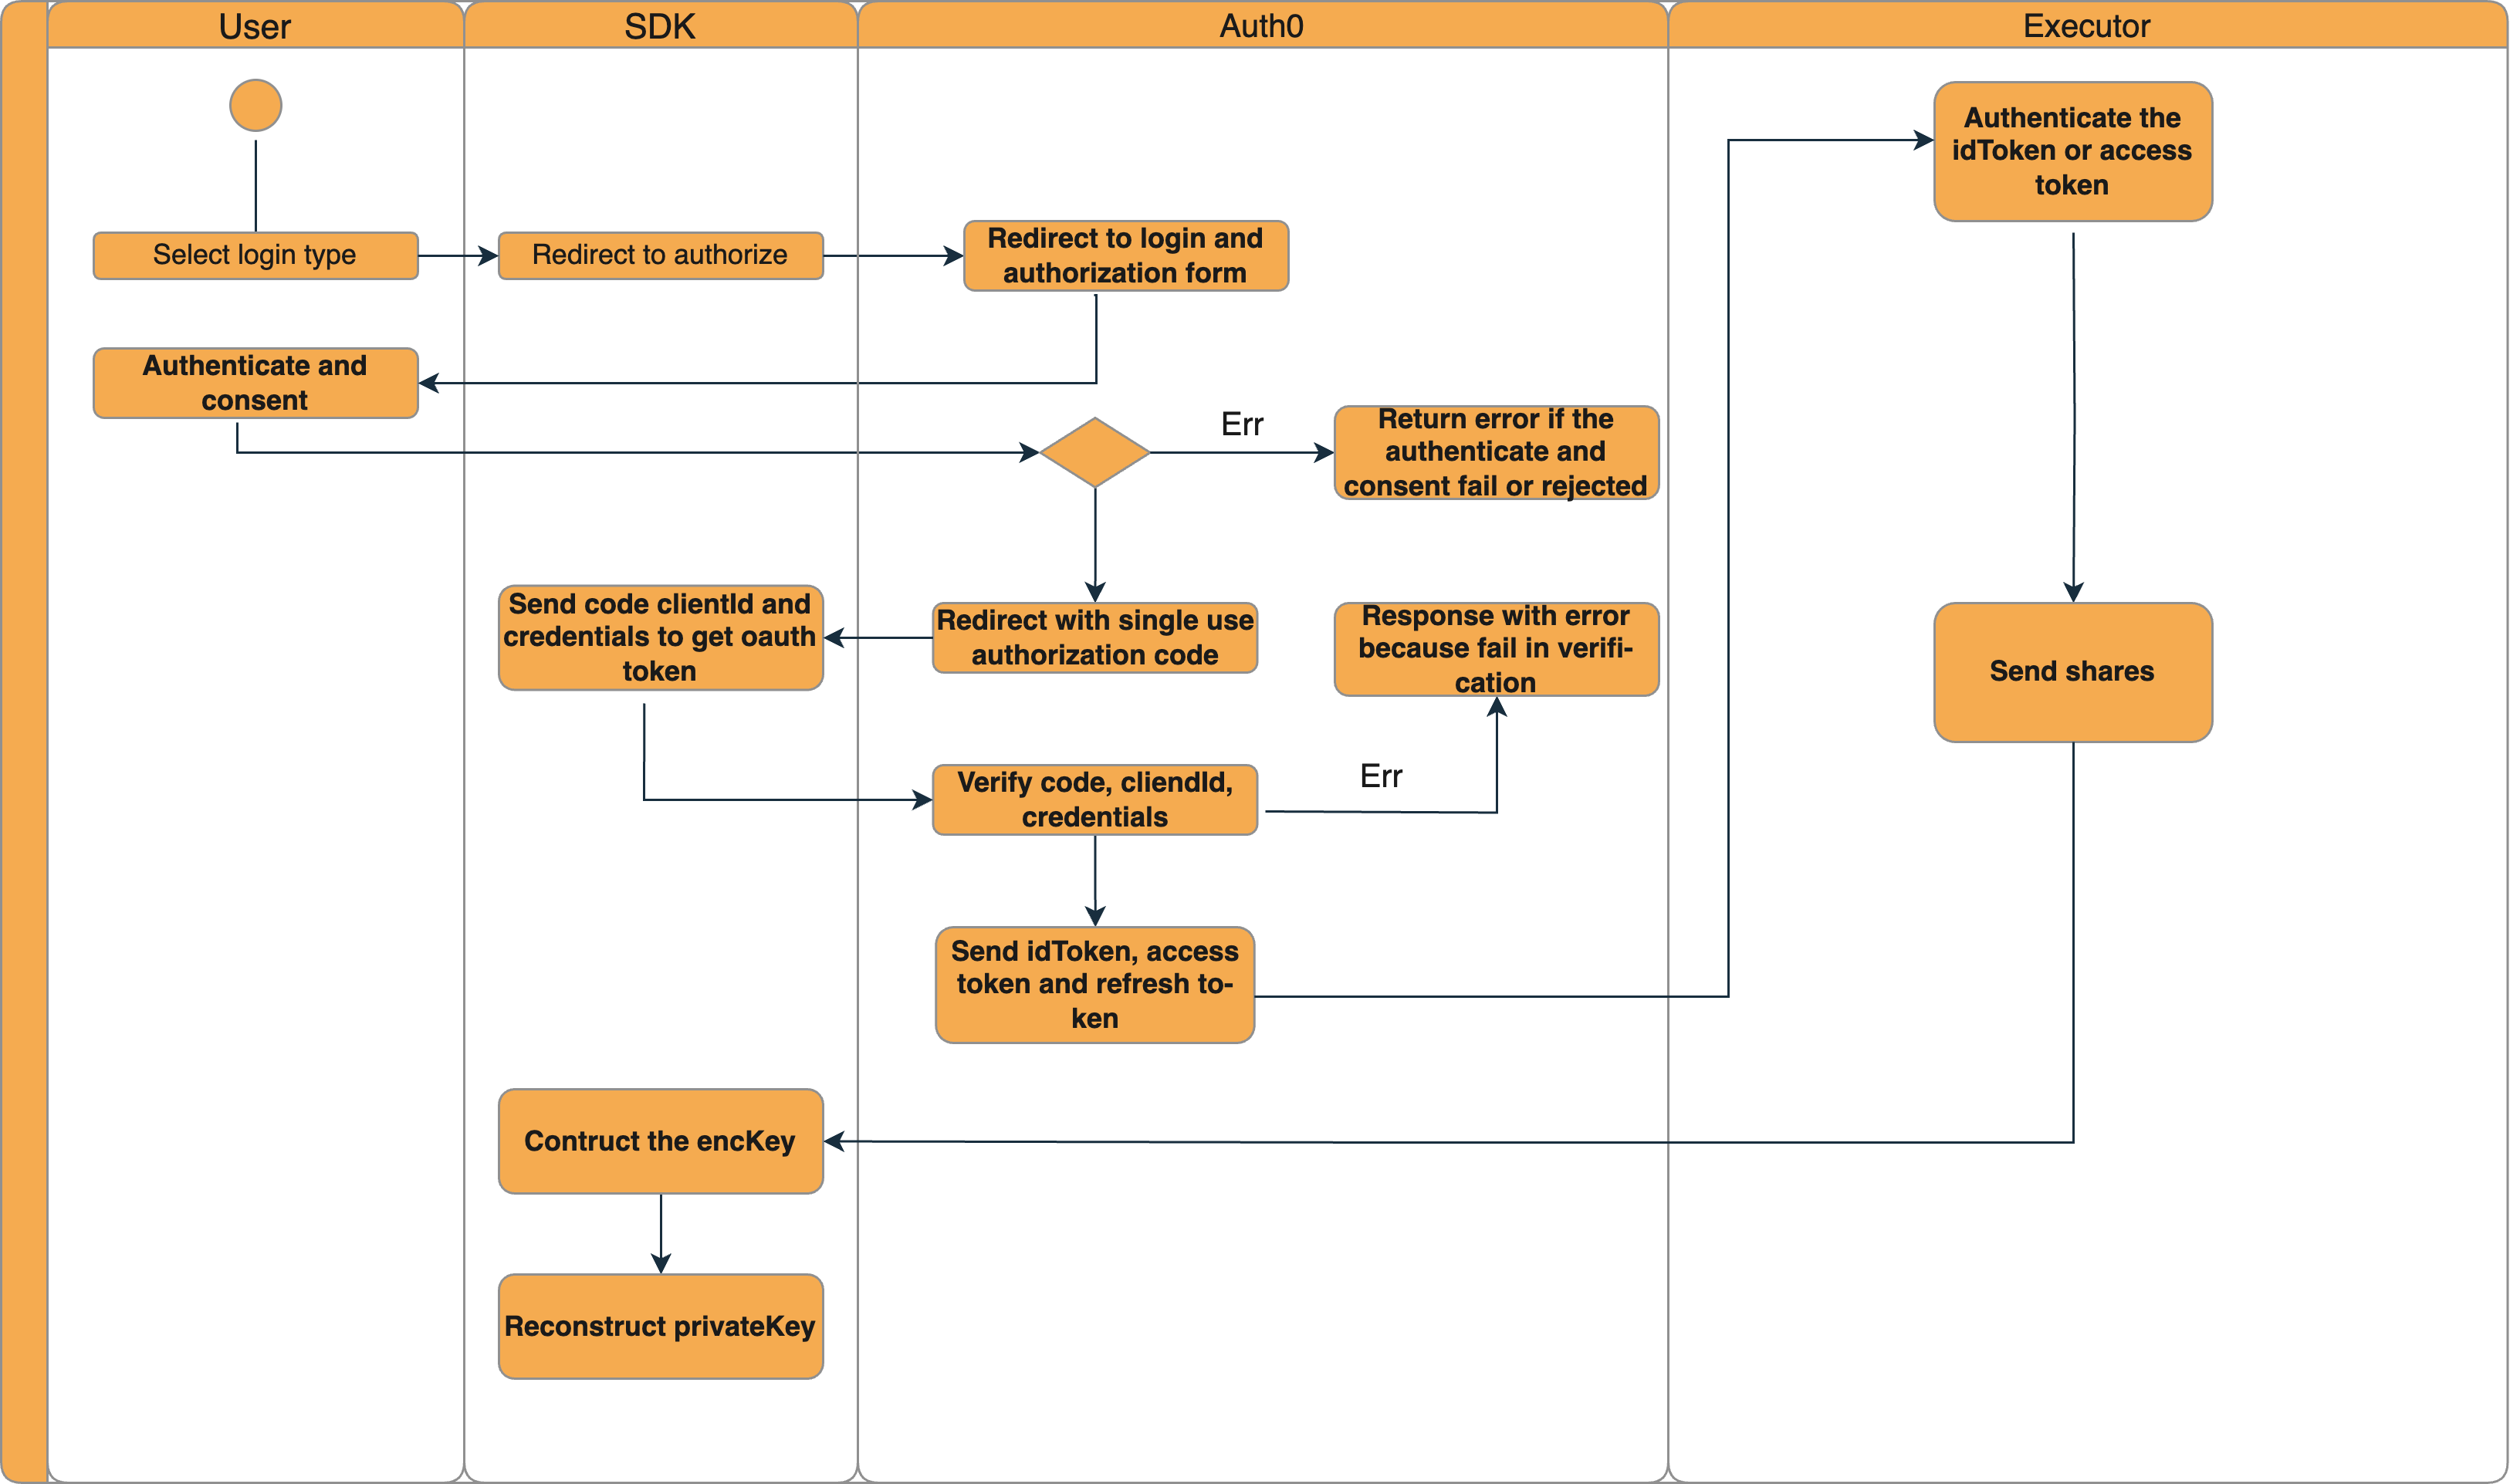
\includegraphics[scale=0.14]{Figure/sign-in-activity.png}
     \caption{Signing in activity}
        \label{fig:sign-in-activity}
    \end{figure}
    Similar to figure \ref{fig:sign-up-activity}, figure \ref{fig:sign-in-activity} describes in detail how users login into the system and how the system's components interact. 

    \begin{table}[H]
      \centering
      \begin{tabular}{|
      >{\columncolor[HTML]{32CB00}}l |lll|}
      \hline
      \textbf{Usecase code}       & \multicolumn{1}{l|}{UC001} & \multicolumn{1}{l|}{\textbf{Usecase name}} & Social login \\ \hline
      \textbf{Actor}              & \multicolumn{3}{l|}{User}                                                              \\ \hline
      \textbf{Pre-condition}       & \multicolumn{3}{l|}{At least have 1 social account}                                    \\ \hline
      \textbf{Main flow of event} & \multicolumn{3}{l|}{
                \begin{tabular}{|
                  >{\columncolor[HTML]{FFFFFF}}p{2cm}|p{3cm}|p{6cm}|}
                      \hline
                      \cellcolor[HTML]{F56B00}\textbf{No} & \cellcolor[HTML]{F56B00}\textbf{Actor} & \cellcolor[HTML]{F56B00}\textbf{Action} \\ \hline
                      \textbf{1}                          & User                                   &  Select social login type    \\ \hline
                      \textbf{2}                          & System                                       &  Redirect to authorize\\ \hline
                      \textbf{3}                          & Auth0                                       &  Redirect to login and authorization form  \\ \hline
                      \textbf{4}                          & User                                       & Authenticate and consent                                         \\ \hline
                      \textbf{5}                          & Auth0                                       & Redirect with single use authorization code\\ \hline
                      \textbf{6}                          & System                                  & Send code clientId and credentials to get oauth token\\ \hline
                      \textbf{7}                          & Auth0                                   & Verify code, cliendId, credentials \\ \hline
                      \textbf{8}                          & Auth0                                   & Send idToken, access token and refresh token\\ \hline
                      \textbf{9}                          & System                                  & Authenticate the idToken or access token\\ \hline
                      \textbf{10}                          & System                                  & Send shares \\ \hline
                      \textbf{11}                          & System                                  & Contruct the encKey \\ \hline
                      \textbf{12}                          & System                                  & Query metadata\\ \hline
                      \textbf{13}                          & System                                  & Return shares description\\ \hline
                      \textbf{14}                          & System                                  & View private key and share description\\ \hline
                \end{tabular}
      } \\ \hline
      \textbf{Alternative flow of event} & \multicolumn{3}{l|}{
                \begin{tabular}{|
                  >{\columncolor[HTML]{FFFFFF}}p{2cm}|p{3cm}|p{6cm}|}
                      \hline
                      \cellcolor[HTML]{F56B00}\textbf{No} & \cellcolor[HTML]{F56B00}\textbf{Actor} & \cellcolor[HTML]{F56B00}\textbf{Action} \\ \hline
                      \textbf{5b}                          & Auth0    &  Return error if the authenticate and consent fail or rejected\\ \hline
                      \textbf{8b}                          & Auth0    &  Response with error because fail in verification\\ \hline
                \end{tabular}
      }
      \end{tabular}
        \caption{View private key and shares description}
        \label{view-pv-shares}
      \end{table}
      \begin{figure}[H]
       \centering
       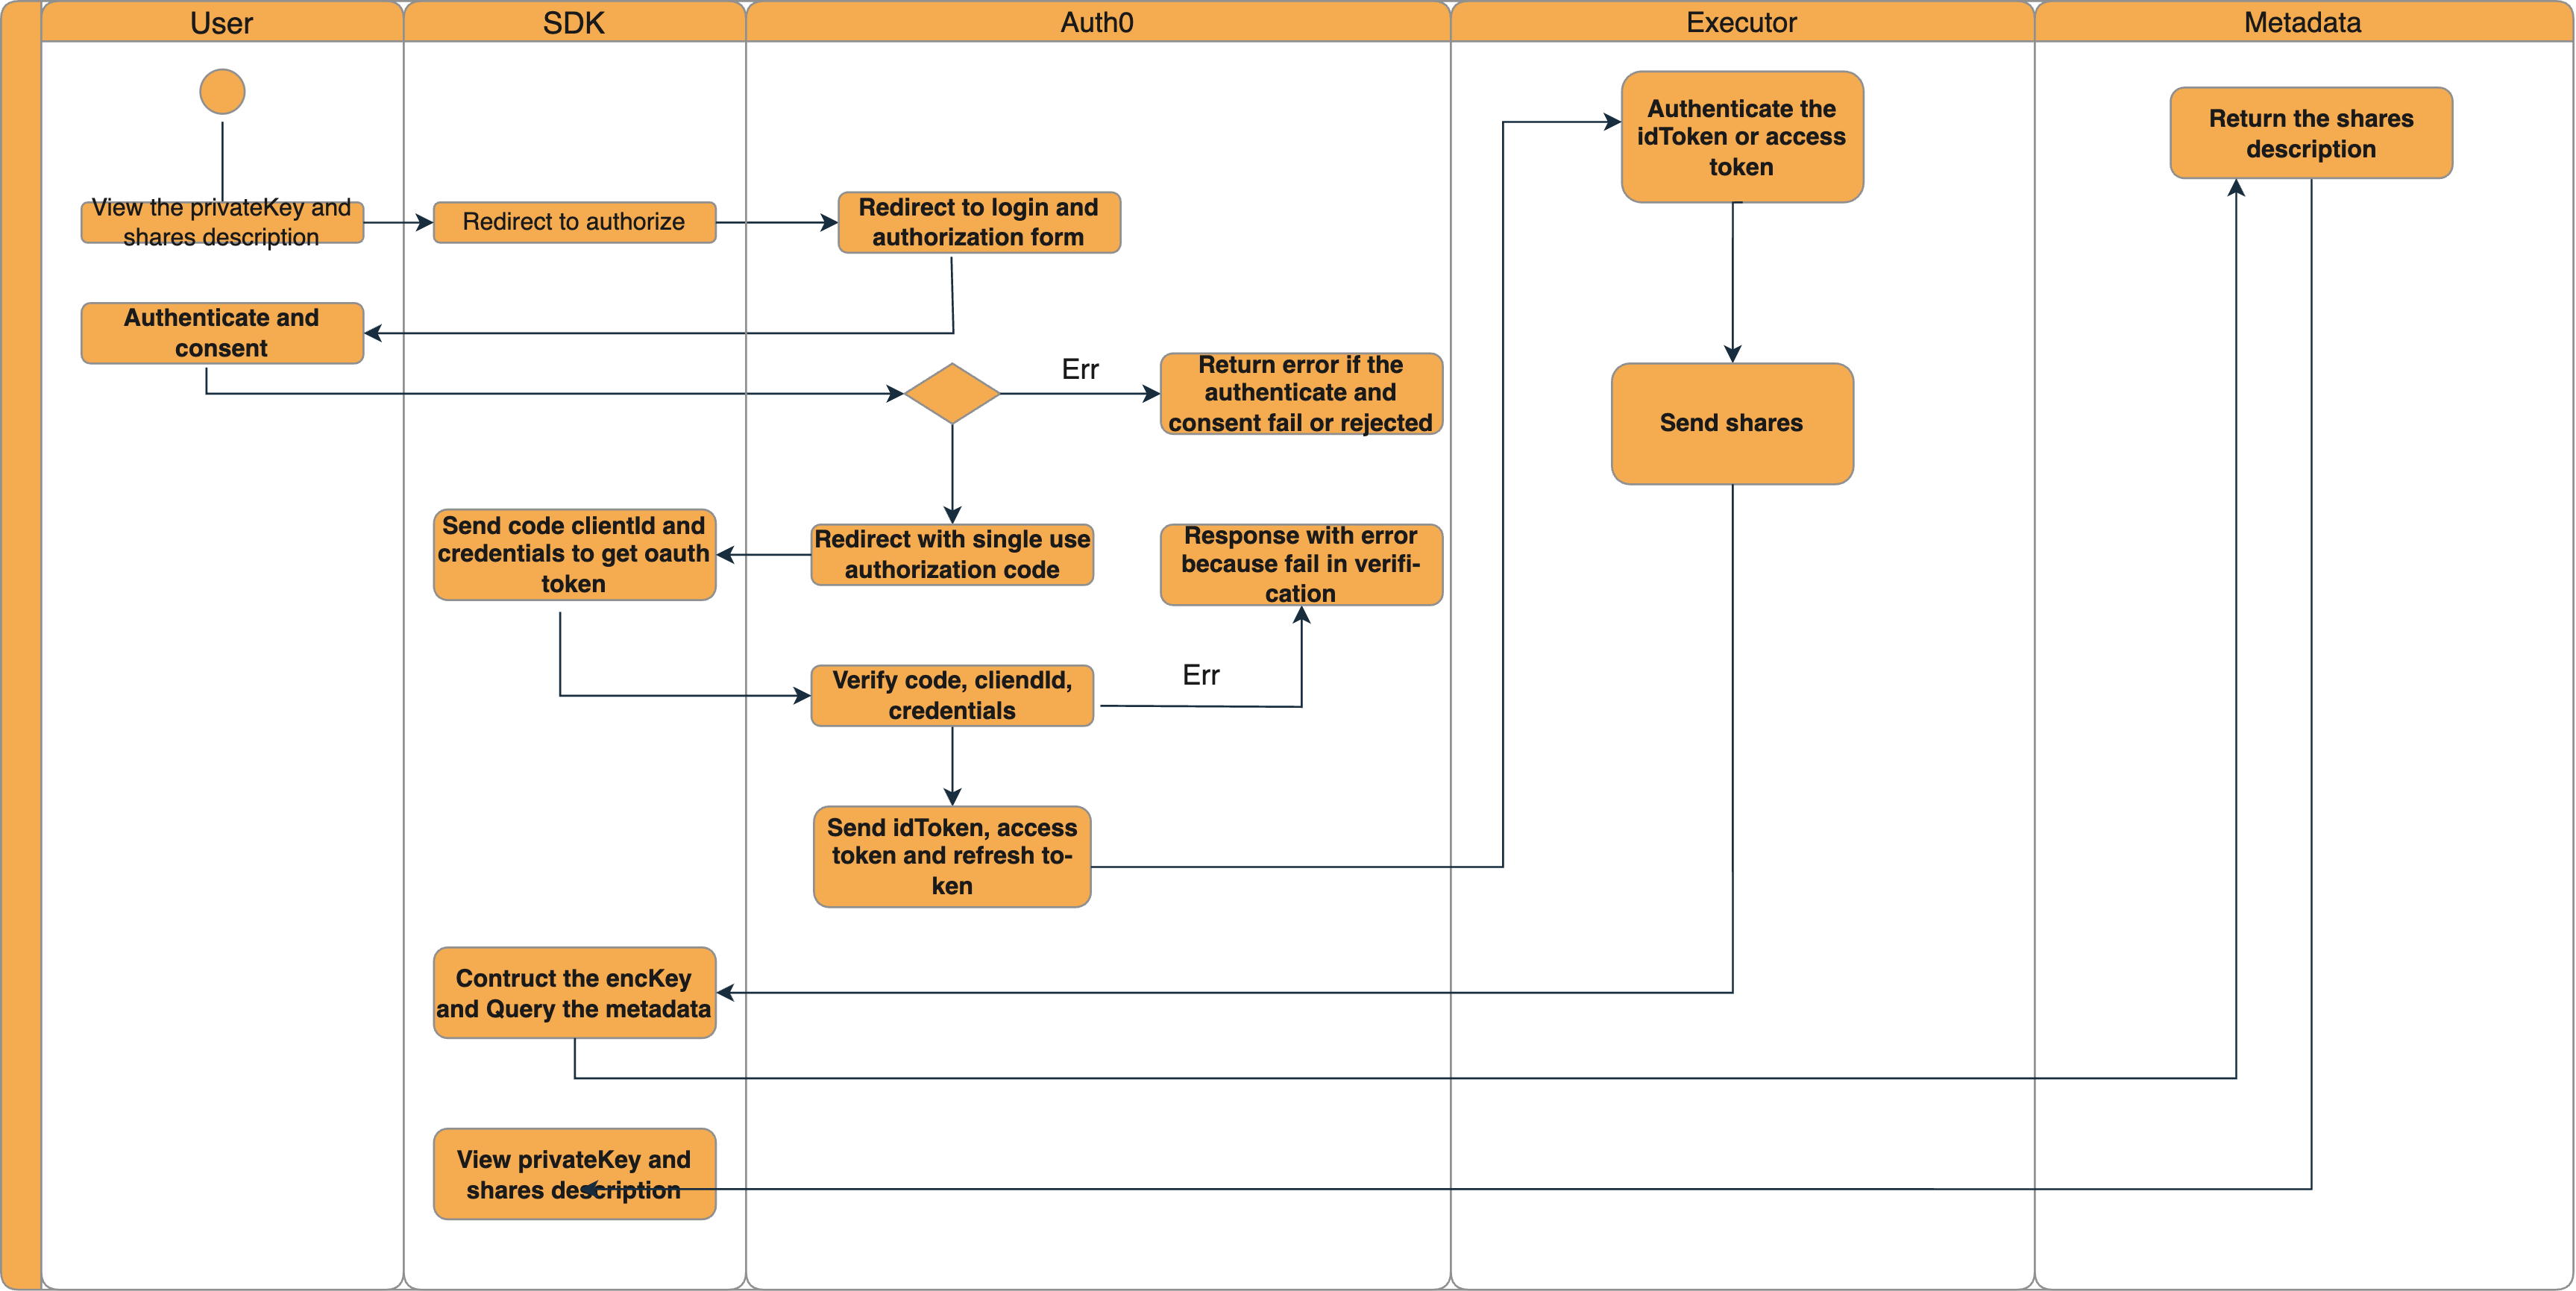
\includegraphics[scale=0.14]{Figure/view-pv-shares-activity.png}
       \caption{View private key and shares description activity}
          \label{fig:view-pv-shares-activity}
      \end{figure}


\end{document}
